% une phrase par ligne, une ligne par phrase
% le label des équations : "eq:Ch08-0xx"
% figure : \includegraphics{../images/T1_Ch08-0x}
% référence à une équation avec \eqref
% référence aux sections et au paragraphes \ref{ssec:Ch0X-y.z} ; y : section ; z : ss-section ; si référence à y sec au lieu de ssec ; si référence à tout le chapitre mettre chap 

\chapter{Problèmes plans en élasticité}\label{chap:Ch08}
\section{Élasticité plane}\label{sec:Ch08-1}
\subsection{Déformations planes}\label{ssec:Ch08-1.1}
Dans de nombreux problèmes, on peut supposer les déformations planes.
\begin{equation}
    u_1=u_1(x_1,x_2), u_2=u_2(x_1,x_2), u_3=0
    \label{eq:Ch08-001}
\end{equation}
On en tire le tenseur des déformations 
\begin{equation}
    \tens{\varepsilon}=
    \begin{bmatrix}
        \varepsilon_{11} & \varepsilon_{12} & 0 \\
        \varepsilon_{12} & \varepsilon_{22} & 0 \\
        0                & 0                & 0 \\     
    \end{bmatrix}
    \quad
    \begin{aligned}
         \varepsilon_{11}&= u_{1,1} \\
         \varepsilon_{22}&= u_{2,2} \\
         \varepsilon_{12}&= \frac{1}{2}(u_{1,2}+u_{2,1} 
    \end{aligned}
\label{eq:Ch08-002}
\end{equation}
et, par la loi de comportement, le tenseur des contraintes
\begin{equation}
    \tens{\sigma} =
    \begin{bmatrix}
        \sigma_{11} & \sigma_{12} & 0           \\
        \sigma_{12} & \sigma_{22} & 0           \\
        0           & 0           & \sigma_{33} \\     
    \end{bmatrix}
\label{eq:Ch08-003}
\end{equation}
avec les relations suivantes :
\begin{equation}
   \begin{cases}
     E\varepsilon_{11} = \sigma_{11}-\nu(\sigma_{22}+\sigma_{33}) \\
     E\varepsilon_{22} = \sigma_{22}-\nu(\sigma_{11}+\sigma_{33}) \\
     E\varepsilon_{12} = (1+\nu)\sigma_{12}
   \end{cases}
    \label{eq:Ch08-004}
\end{equation}
\begin{equation}
     E\varepsilon_{33} = 0 = \sigma_{33}-\nu(\sigma_{11}+\sigma_{22})
    \label{eq:Ch08-005}
\end{equation}
L'équation \eqref{eq:Ch08-005} donne alors
\begin{equation}
    \sigma_{33}=\nu(\sigma_{11}+\sigma_{22})
    \label{eq:Ch08-006}
\end{equation}
et en reportant dans \eqref{eq:Ch08-004} il vient 
\begin{equation}
   \begin{cases}
     E\varepsilon_{11} = (1-\nu^2)\sigma_{11} - \nu(1+\nu)\sigma_{22}\\
     E\varepsilon_{22} = (1-\nu^2)\sigma_{22} - \nu(1+\nu)\sigma_{11}\\
     E\varepsilon_{12} = (1+\nu)\sigma_{12}
   \end{cases}
    \label{eq:Ch08-007}
\end{equation}

Pour résoudre un problème en déformations planes, il faut trouver les déplacements $u_1$, $u_2$ et les contraintes $\sigma_{11}$, $\sigma_{22}$, et $\sigma_{12}$ en fonction des coordonnées $(x_1,x_2)$ dans le plan.
Si nous travaillons sur les contraintes, c'est-à-dire en utilisant l'approche du paragraphe~\ref{ssec:Ch06-1.4}, il faudra vérifier les équations d'équilibre et les équations de Beltrami. 
Les équations d'équilibre s'écrivent 
\begin{equation}
   \begin{cases}
     \sigma_{11,1}+\sigma_{12,2}=0\\
     \sigma_{12,1}+\sigma_{22,2}=0
   \end{cases}
    \label{eq:Ch08-008}
\end{equation}
en supposant nulles les forces de volume (sinon, l'analyse qui suit peut s'étendre, avec des résultats plus compliqués). 
Ces équations expriment que les formes 
\begin{equation*}
\sigma_{11}dx_2-\sigma_{12}dx_1 \qquad,\qquad \sigma_{22}dx_1-\sigma_{12}dx_2
\end{equation*}
sont des différentielles totales. Il existe donc deux fonctions   $\varphi{x_1,x_2}$ et $\psi(x_1,x_2)$ telles que 
\begin{equation*}
\sigma_{11}=\varphi_{,2} \qquad \sigma_{12}=-\psi_{,2}=-\varphi_{,1} \qquad \sigma_{22}=\psi_{,1}
\end{equation*}

En comparant les deux expressions de $\sigma_{12}$, on voit que la forme 
\begin{equation*}
\psi dx_1 + \varphi dx_2
\end{equation*}
est une différentielle totale, il existe donc une fonction $\chi(x_1,x_2)$ telle que 
\begin{equation*}
\varphi=\chi_{,2} \qquad \psi=\chi_{,1}
\end{equation*}

La fonction $\chi(x_1,x_2)$ est appelée «~fonction d'Airy~» ou «~fonction de contraintes~» du problème. 
Elle permet de calculer les contraintes par 
\begin{equation}
\sigma_{11}=\chi_{,22} \qquad \sigma_{12}=\chi_{,12} \qquad \sigma_{22}=\chi_{,11}
    \label{eq:Ch08-009}
\end{equation}

les équations de l'équilibre étant alors automatiquement vérifiées. 
En remarquant que, d'après \eqref{eq:Ch08-006} et \eqref{eq:Ch08-009}, 
\begin{equation}
\sigma_{kk}=(1+\nu)(\sigma){11}+\sigma_{22}=(1+\nu)\Delta\chi
\label{eq:Ch08-010}
\end{equation}
les équations de Beltrami \ref{sec:Ch6-31} donnent 
\begin{equation}
  \begin{aligned}
  i,j = 1,1 & : &  (1+\nu) \Delta\chi_{,22} + (1+\nu) \Delta\chi_{,11}=0 \\
        2,2 & : &  (1+\nu) \Delta\chi_{,11} + (1+\nu) \Delta\chi_{,22}=0 \\ 
        1,2 & : & \cancel{-(1+\nu) \Delta\chi_{,12}} + \cancel{(1+\nu) \Delta\chi_{,12}}=0 \\
        3,3 & : & \nu(1+\nu) \Delta\Delta\chi = 0 \\
  \end{aligned}
\label{eq:Ch08-011}
\end{equation}

Toutes ces équations seront vérifiées si et seulement si la fonction $\chi$ est biharmonique 
\begin{equation}
\Delta\Delta\chi=\chi_{,1111}+2\chi_{,1122}+\chi_{,2222}=0
\label{eq:Ch08-012}
\end{equation}
Ainsi, pour résoudre un problème en déformations planes, il faut trouver une fonction de contraintes $\chi$ biharmonique vérifiant les conditions aux limites. 
On en tire alors les contraintes $\sigma_{11}$, $\sigma_{22}$ et $\sigma_{12}$ par \eqref{eq:Ch08-009}, $\sigma_{33}$ par \eqref{eq:Ch08-006}, les déformations par \eqref{eq:Ch08-007} et les déplacements par intégration du système 
\begin{equation}
  \begin{cases}
  \varepsilon_{11}=u_{11}=\frac{1+\nu}{E}[(1-\nu)\chi_{,22}-\nu\chi_{,11}] \\
  \varepsilon_{22}=u_{22}=\frac{1+\nu}{E}[(1-\nu)\chi_{,11}-\nu\chi_{,22}] \\
  2\varepsilon_{12}=u_{12}+u_{21}=\frac{2(1+\nu)}{E}\chi_{,12}
  \end{cases}
\label{eq:Ch08-013}
\end{equation}
système qui est intégrable puisque les équations de Beltrami sont vérifiées. 
\subsection{Contraintes planes}\label{ssec:Ch08-1.2}
L'hypothèse des déformations planes convient pour une pièce suffisamment longue pour que l'on puisse négliger la déformation longitudinale. 
Pour une plaque mince, chargée dans son plan, la condition aux limites pour 
\begin{center}
    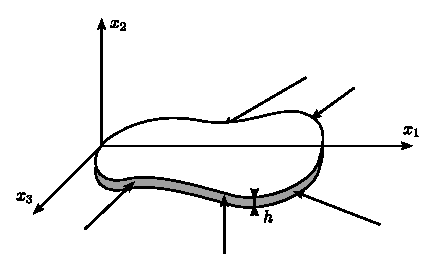
\includegraphics{../images/T1_Ch08-01}
\end{center}
$x_3=\pm h/2$ donne 
\begin{equation}
  x3 = \pm \frac{h}{2} : \qquad \sigma_{13}=\sigma_{23}=\sigma_{33}=0
\label{eq:Ch08-014}
\end{equation}
et on recherche donc un état de contraintes planes 
\begin{equation}
  \tens{\sigma}=\begin{bmatrix}
     \sigma_{11}(x_1,x_2) & \sigma_{12}(x_1,x_2) & 0 \\
     \sigma_{12}(x_1,x_2) & \sigma_{22}(x_1,x_2) & 0 \\
      0                   &  0                   & 0 
   \end{bmatrix}
\label{eq:Ch08-015}
\end{equation}
Le tenseur des déformations est donné par
\begin{equation}
  \tens{\varepsilon} = \begin{bmatrix}
     \varepsilon_{11} & \varepsilon_{12} & 0           \\
     \varepsilon_{12} & \varepsilon_{22} & 0           \\
      0               &  0               & \varepsilon_{33} 
   \end{bmatrix}
\label{eq:Ch08-016}
\end{equation}
\begin{equation}
    \begin{cases}
        E \varepsilon_{11} & = \sigma_{11}-\nu\sigma_{22}\\
        E \varepsilon_{22} & = \sigma_{22}-\nu\sigma_{11}\\
        E \varepsilon_{33} & = -\nu (\sigma_{11}+\sigma_{22})\\
        E \varepsilon_{12} & = (1+\nu)\sigma_{12}
    \end{cases}
    \label{eq:Ch08-017}
\end{equation}
Les équations d'équilibre se traitent comme en déformations planes et conduisent à \eqref{eq:Ch08-009}. 
On a alors 
\begin{equation}
  \sigma_{kk}=\sigma_{11}+\sigma_{22}=\Delta\chi
\label{eq:Ch08-018}
\end{equation}
et les équations de Beltrami donnent 
\begin{equation}
  \begin{cases}
    i,j=1,1  &  (1+\nu) \Delta\chi_{,22}+\Delta\chi_{,11} = 0\\
    i,j=2,2  &  (1+\nu) \Delta\chi_{,11}+\Delta\chi_{,22} = 0\\
    i,j=1,2  & -(1+\nu) \Delta\chi_{,12}+\Delta\chi_{,12} = 0
  \end{cases}
\label{eq:Ch08-019}
\end{equation}
équations qui ne pourront être vérifiées que si $\Delta\chi$ est fonction linéaire des coordonnées, ce qui est bien trop restrictif pour permettre de résoudre des problèmes réels.
Nous oublions donc provisoirement les équations de Beltrami, et nous allons chercher à calculer les déplacements à partir de \eqref{eq:Ch08-017} 
\begin{equation*}
  E\varepsilon_{11}=\chi_{,22}+\nu\chi_{,11}=(1+\nu)\chi_{,22}-\nu\Delta\chi
\end{equation*}
et finalement on obtient 
\begin{equation}
  \begin{cases}
    \varepsilon_{11}   &  = u_{1,1} = (1+\nu) \Delta\chi_{,22}+\Delta\chi_{,11} = 0\\
    \varepsilon_{22}   &  = u_{2,2} =   (1+\nu) \Delta\chi_{,11}+\Delta\chi_{,22} = 0\\
    2\varepsilon_{12}  &  = u_{1,1} =  -(1+\nu) \Delta\chi_{,12}+\Delta\chi_{,12} = 0
  \end{cases}
\label{eq:Ch08-020}
\end{equation}
\begin{equation*}
  E\varepsilon_{11}=\chi_{,22}+\nu\chi_{,11}=(1+\nu)\chi_{,22}-\nu\Delta\chi
\label{eq:Ch08-021}
\end{equation*}
Le système \eqref{eq:Ch08-020} est formellement identique au système \eqref{eq:Ch08-020} en remplaçant $\nu$ par $\nu/(1+\nu)$.
Il permettra donc de calculer $u_1(x_1,x_2)$ et $u_2(x_1,x_2)$ si et seulement si la fonction $\chi$ est biharmonique.
Il reste à intégrer les équations \eqref{eq:Ch08-021} pour calculer $u_3$ 
\begin{equation}
  \varepsilon = - \frac{\nu}{E} \quad \Rightarrow \quad u_3 = - \frac{\nu}{E} \Delta \chi(x_1,x_2)x_3+a(x_1,x_2)
\label{eq:Ch08-022}
\end{equation}
\begin{equation}
  \begin{cases}
     2 \varepsilon_{13} & = u_{3,1}+u_{1,3}=-\frac{\nu}{E} \Delta \chi_{,1}x_3+a_{,1} = 0 \\
     2 \varepsilon_{23} & = u_{3,2}+u_{2,3}=-\frac{\nu}{E} \Delta \chi_{,2}x_3+a_{,2} = 0
  \end{cases}
\label{eq:Ch08-023}
\end{equation}
équations qui ne pourront jamais être vérifiées puisque $a$ et $\chi$ ne dépendent que de $x_1$ et $x_2$. 
Ainsi, si $\chi$ est biharmonique, on ne peut pas calculer les déplacements ; c'est tout à fait normal, puisque les équations de Beltrami \eqref{eq:Ch08-019} donnent 
\begin{equation}
  \Delta \chi(,11) = \Delta \chi(,22) = \Delta \chi(,12) = 0
\label{eq:Ch08-024}
\end{equation}
conditions que nous avons volontairement laissées de côté.
Cependant, pour une plaque mince, $x_3$ est petit, et en première approximation, \eqref{eq:Ch08-023} donne $a_{,1}=a_{,2}=0$, $a=Cste$ et la solution ainsi construite est une approximation satisfaisante de la réalité : c'est l'approximation «~contraintes planes~».
 
Ainsi, en déformations planes comme en contraintes planes, la solution est donnée par une fonction de contraintes $\chi(x_1,x_2)$ biharmonique, donnant les contraintes par \eqref{eq:Ch08-019} et les déplacements $u_1(x_1,x_2)$ et $u_2(x_1,x_2)$ par inté­gration du système
\begin{equation}
  \begin{cases}
    u_{1,1} & =\frac{1+\nu}{E}\{ \chi_{,22}+ r \Delta \chi \} \\
    u_{2,2} & =\frac{1+\nu}{E}\{ \chi_{,11}+ r \Delta \chi \} \\
    u_{1,2} & + u_{2,1} = -\frac{2(1+\nu)}{E}\chi_{,12}
  \end{cases}
\label{eq:Ch08-025}
\end{equation}
\begin{equation*}
  \text{avec} \quad \left| 
  \begin{aligned}
    r & = \nu \text{ en déformations planes} \\
    r & = \nu / (1+\nu) \text{ en contraintes planes}
  \end{aligned}
  \right.
\end{equation*}
De plus, en déformations planes, la contrainte axiale $\sigma_{33}$ est donnée par \eqref{eq:Ch08-006}, tandis que, en contraintes planes, la variation d'épaisseur de la plaque mince est donnée par \eqref{eq:Ch08-022} 
\begin{equation}
u_3 = -\frac{\nu}{E}\Delta\chi
\label{eq:Ch08-026}
\end{equation}

\subsection{Utilisation de la variable complexe} \label{ssec:Ch08-1.3}
Introduisons la variable complexe 
\begin{equation}
  z=x_1+\imath x_2 \qquad \bar{z}=x_1-\imath x_2
\label{eq:Ch08-027}
\end{equation}
\newtheorem*{TRep}{Théorème de la représentation}
\begin{TRep}
Toute fonction réelle harmonique peut s'écrire sous la forme 
\begin{equation}
  \varphi(x_1,x_2)=\Re \[F(z)\]
\label{eq:Ch08-028}
\end{equation}
Toute fonction réelle biharmonique peut s'écrire sous la forme 
\begin{equation}
  \chi(x_1,x_2)=\Re \[\bar{z}G(z)+K(z)\]
\label{eq:Ch08-029}
\end{equation}
avec $F$ , $G$ et $K$ fonctions holomorphes. 
\end{TRep}
\\
\begin{proof}
La première représentation est classique: on sait que les parties réelle et imaginaire d'une fonction holomorphe sont deux fonctions harmoniques con­juguées, c'est-à-dire reliées par les conditions de Cauchy 
(30) 
\begin{equation}
  \begin{cases}
    \varphi(z)=P(x_1,x_2)+\imath Q(x_1,x_2) \\
    P_{,1}=Q_{,2} \quad , \quad P_{,2}=Q_{,1}
  \end{cases}
\label{eq:Ch08-030}
\end{equation}
La seconde représentation peut s'obtenir à partir de la précédente par deux méthodes. \\
1ère méthode. À partir de \eqref{eq:Ch08-027}, on voit que toute fonction de $(x_1,x_2)$ peut être considérée comme fonction de $(z,\bar{z})$. 
On obtient alors facilement 
\begin{equation*}
  \Delta \varphi = \frac{\partial^2\varphi}{\partial x_1^2} + \frac{\partial^2\varphi}{\partial x_2^2} = \frac{\partial^2\varphi}{\partial z \partial \bar{z}}
\end{equation*}
de sorte que si $\varphi$ est biharmonique
\begin{equation*}
  \Delta\Delta\varphi=\frac{\partial^4\varphi}{\partial^2 z \partial^2 \bar{z}}=0
\end{equation*}
on obtient $\varphi=\bar{z}F_1(z)+G_1(z)+zF_2(\bar{z})+G_2(\bar{z})$ \\
et en écrivant que $\varphi$ est réelle, on obtient \eqref{eq:Ch08-029}.\\
2ème méthode. Si $\chi$ est biharmonique, la fonction $p=\Delta\chi$ est harmonique, et on peut écrire 
\begin{equation*}
  p=\Re \[ g(z)\]
\end{equation*}
Nous introduisons la fonction 
\begin{equation*}
  G(z) = \frac{1}{4}\int g(z) dz = P + \imath Q
\end{equation*}
avec $p=4P_{,1}=4Q_{,2}$.
On obtient alors 
\begin{equation*}
  \Delta (\chi - Px_1 + Qx_2) = \Delta\chi - 2P_{,1} - 2Q_{,2} = \Delta\chi - p = 0
\end{equation*}
et la fonction $\chi - Px_1 + Qx_2$, est harmonique, d'où
\begin{equation*}
  \begin{aligned}
    \chi & = Px_1 + Qx_2 + \Re \[ K(z)\]\\
         & = \Re \[\bar{z}G(z) + K(z) \]   \qquad \text{cqfd} 
\end{equation*}
\end{proof}

L'application de ce théorème montre que la fonction de contrainte d'un problème d'élasticité plane est déterminée par deux fonctions holomor­phes $G$ et $K$.
On posera 
\begin{equation}
  \begin{cases}
    G    & = P + \imath Q \\
    K    & = R + \imath S \\
    \chi & = Px_1 + Qx_2 + R
  \end{cases}
\label{eq:Ch08-031}
\end{equation}
et les relations \eqref{eq:Ch08-009} donneront 
\begin{equation}
  \begin{cases}
    \sigma_{11} & = P_{,22} x_1 + Q_{,22} x_2 + 2 Q_{,2} + R_{,22} \\
    \sigma_{22} & = P_{,11} x_1 + Q_{,11} x_2 + 2 P_{,1} + R_{,11} \\
    \sigma_{12} & = Q_{,11} x_1 - P_{,11} x_2 + S_{,11}
  \end{cases}
\label{eq:Ch08-032}
\end{equation}
En regroupant et en utilisant les relations de Cauchy \eqref{eq:Ch08-030}, on obtient 
\begin{equation}
  \begin{cases}
    \sigma_{11} + \sigma_{22} = 4 \Re \[G'(z)\] \\
    \sigma_{22} - \sigma_{11} + 2 \imath \sigma_{12} = 2 \[\bar{z}G''(z) + K''(z) \]
  \end{cases}
\label{eq:Ch08-033}
\end{equation}
L'intégration de \eqref{eq:Ch08-025} donne également 
\begin{equation}
  \begin{cases}
    u_1 & = \frac{1+\nu}{E}\{(3-4r)P - P_{,1}x_1 - Q_{,1}x_2 - R_{,1} + Cx_2 + \alpha \}\\
    u_2 & = \frac{1+\nu}{E}\{(3-4r)Q - Q_{,1}x_1 - P_{,1}x_2 - S_{,1} + Cx_1 + \beta \}\\
  \end{cases}
\label{eq:Ch08-034}
\end{equation}
ou sous forme complexe 
\begin{equation}
  \frac{E}{1+\nu}(u_1 + \imath u_2) & = (3-4r)G(z) - z\overline{G'(z)} - \overline{K'(z)} - \imath C z + \alpha +\imath\beta
\label{eq:Ch08-035}
\end{equation}
les trois derniers termes représentant le mouvement de solide. 
Ces représen­tations sont à la base de la théorie de l'élasticité plane qui permet de pous­ser très loin les calculs (voir \cite{Muskhelishvili-53}). 
Nous présenterons simplement quelques exemples.

\section{Exemples d'applications}\label{sec:Ch08-2}
\subsection{Problème de Saint-Venant}\label{ssec:Ch08-2.1}
\endinput 
Une classe de solutions s'obtient en prenant pour X un polynôme homogène de degré n, .OU, ce qUi revient au même, 

On obtient ainsi pour tout entier TI une solution dépendant de 4 constantes. 
n=2 ! Un polynôme du second degré est automatiquement biharmonique, et con­duit à un état de contraintes constant 
'X ~ 1t IX. l:1.:,t .. Z f.> 1:>-,1:>-" .,. ~ x,," 1 
(37) 
[ 
a:;~ = t (J"tl, : 01 cr:,l, : -~ 
~ : Un polynôme du 3ème degré est aussi automatiquement biharmonique, et conduit à un état de contraintes linéaire 
-t
'X = { a. 1:1.:, ~ + ~ t. ~:oc" + ~ C-IX, oc~ + .d. X; 1 
G 
(38~ 
{ (\""\0\ =-c 1:1.:, + <toc./, <fJ.1, = a..~, + k'X../, (f"l-= -(k -:x., + ,c >:Cl,) 
-128 ­
n=4 Pour un polynôme du 4ème degré, on a 
~ 3 	t 1, ~ 
'X = 	~ tAIX, + J, B'l:.~ /.t2" -?> (A + 1») ~1 1.tJ, +.t C/.t,ft}, + 1> ();l." 1 cr-= -(A .. 1») 'L+ .l, c 'l:., 'l:.J, + 1, J> x;
f 	t 
(39) 'H 	1 
2, A 'LI, 	_ ( A <Il) IX.,t,
<T!LJ,= ~ + 1, B~I.t,t, ,t,l /.t1, C 1,
cr:;Q,~ -P-> + J., (A ... D)~• ./l:J, -4"
1 
et ainsi de suite. A titre d'application, montrons qu'une superposition de solutions de ce type permet de résoudre le problème de Saint-Venant en contraintes ou 

e. 
Le matériau occupe le rectangle [0,2] x[-{/~J t-/l]; la surface latérale «-l,=:!:f./:t est libre de contrainte, et les extrémités x)=O et x = l sont soumises à
l 
deux torseurs plans en équilibre (voir § VII.I. 1). Les conditions aux limi­teS sont donc, sur la surface latérale 

et sur l'extrémité x I= l 

Bien entendu, comme nous l'avons discuté au § VII.I.I, ce problème admet plusieurs solutions, et nous allons chercher s'il en existe une correspondant à une fonction de contrainte X(1:t.4: ) polynôme non homogène du 4ème degré,
11 1I
càd 	superposition de (37),(38) et (39). La condition aux limites (40) donne 

relations qU1 doivent être vérifiées pour tout Il vient
xI' 
~ 
= e, 	: 0 , a..=lr.O e, = A .. 'D 0 Jr s oC = 0 
(43) 
lA cl. -(A+ 1» ,!t = 0 {:> + C _ .l" 0
'" 
4 	4 
(44) C .,:c, ');~ -t-d. -:c~ 1 'X ~ C Yt."
x = --+ -t --/.IC,/.IC~
, " G " l, 4 
cr = .l,C 1.1:. ILJ, .. cl. ACt + t
~~ 
(45) 
O"~'l, = C ( ~" le:)
4 
= 0 
Les trois conditions (41) permettent alors de déterminer les constantes C , cl et r en fonction de 1', Q et M , càd des efforts appliqués 
(46) 

c = 

La répartition des contraintes normales est linéaire, COmme dans le cas général (§ VI.I.2) et la répartition des contraintes tangentielles~" est parabolique. C'est ce que l'on obtiendrait à partir de l'analyse du § VI.3 pour une section rectangulaire très large (déformation, ulanes) ou très étroite (contraintes planes). 
2.2 TRACTION D'UNE PLAQUE PERFOREE 
Pour certaines géométries simples, l'utilisation de la variable complexe permet de construire explicitement la solution d'une vaste classe 
de problèmes. C'est en particulier le cas pour les domaines intérieurs ou extérieurs limités par un cercle. A titre d'exemple, nous allons donner la 
solution qui correspond à la traction d'une plaque perforée. 
'X 4 ~~ 

--+----f-Ar:-o..---+~X1 


Si le rayon Cl. du trou est petit par rapport aux dimensions de la plaque, on peut supposer en première approximation la plaque infinie. Dans le repère (x ,x), l'état de contraintes à l'infini est donc
l 2
(47) or 
= 

ce qui, d'après (33), correspond à 
cr­
(48) ; -r 
. 4 

c'est la solution qui se réalise en l'absence de trou, mais en présence d'un trou cette solution ne vérifie pas les CL sur le trou, qui s'écrivent 
(49) 


en notant c:r",~, (J"Jt.9 ,(J'9ft les composantes du tenseur des contraintes sur le repère (.e. ..... .e.e) associé aux coordonnées cylindriques. Le trou indui t donc dans (48) une perturbation, et on montre qu'alors 

(JO' [ CL'"
(50) 

-r --­
t r 

Les contraintes sont alors données par 
(J""[ é t, 4 
_(À .;. 4IL + 3 CL) ~.2,e 1
(J"II-JI. = 
9-e -~",) 
'1,'" fi} 
4
(j'"
(51) 
(j'Le = ( -1+-ié ~ CL ) Mm. .te 9-",'" '1,4 
é 1
?> CL'"
(J"Q9 = (j" f (À + '1,"') + ( À .. '1.'" ) .c«> .2,e
t 
En particulier, sur le trou on a bien (49) et 

L'état de contraintes sur le bord du trou est un état de traction simple avec une contrainte variant de .. ~ cr" (traction, sur l'axe des xl) à a~ (compression, sur l'axe des xZ). La contrainte maximale est trois fois plus grande que la contrainte à l'infini. C'est un exemple de concen­tration de contrainte: la présence d'un trou, ou plus généralement d'un dé­faut, aussi petit soit-il, cause une augmentation importante des contraintes locales au voisinage du trou. 

